
\section{Linear Optical Quantum Computing}\label{sec:Photonic}
Trapped ion quantum computing has made significant practical advances, however, the fundamental concepts of qubits and entanglement aren't limited to any one particular implementation but rather revolve around a quantum system (or systems). Therefore, this section explores a method using photons to represent qubits and then performs operations on those photons to implement quantum logic gate operations on qubits. Linear Optical Quantum Computing (LOQC) is the name used for photonic quantum computers that make use of classical linear optical tools such as beamsplitters, polarisers, phase shifters, etc. to perform these operations. The significant improvement made by LOQC's is the protocol used to make a photonic quantum computer viable at the large qubit scale; this protocol makes use of quantum teleportation as explained at the end of this section. The first step is to transform photons into qubits.

\subsection{Types of Encoding}
The ways in which a photon can be made to represent a qubit is known as the method of "encoding". Much like the different methods for quantum computing in general, there are many different ways to encode photons to represent qubit states; there exists mixed polarisation encoding, parity encoding etc. For this report will focus on spatial encoding, specifically "dual rail" encoding. 

\subsubsection{Spatial Modes}\label{sec:modes}
Single Rail encoding involves sending a photon down a single rail or cavity; imagine a photon travelling down a wire. The existence of a photon in the rail is representative of a qubit with state $\ket{1}$, whilst nothing but vacuum in the rail is representative of a qubit in state $\ket{0}$. Dual rail encoding is very similar but instead of a single rail/cavity there are two. In this case the rails (sometimes called modes) can be labelled A and B; when a photon is detected in mode A but not B this is representative of a qubit with the state $\ket{0}$. When a photon is detected in mode B but not A this is representative of a quibt with the state $\ket{1}$. \\ What is the difference between these types of encoding? As it turns out, performing 2 qubit gate operations (and then entangling multiple qubits) in a single rail encoded quantum computer is very simple; it involves the use of a linear optical tool called the beamsplitter and the phenomena known as the Hong-Ou-Mandel effect (both of these are discussed in more detail later). However, in a dual-rail representation achieving this deterministically isn't physically possible. Similarly, in the dual rail representation, performing 1 qubit operations is quite simple but it is not physically possible to achieve deterministically in the single rail representation. The rest of this section will have a heavy focus on the dual-rail representation and discuss how non-deterministic, or rather probabilistic, tools are used to create 2 qubit gate operations. It is important to note that mathematically, the horizontal-vertical polarisation representation, as introduced in \cref{sec:superposition}, is identical to the dual rail representation. 


%%%%%%%%%%%%%%%%%%%%%%%%%%%%%%%%%%%%%%%%%%

\subsection{Useful Linear Optical Tools and Single Qubit Representations}
Before going into any of the complex techniques that really support photonic quantum computers as a viable, scalable direction for quantum computers of the future, the report will introduce some of the basic tools that can manipulate photons and by extension, qubits.
\subsubsection{Beamsplitters}

The aptly named beamsplitter divides a beam of light into two. The intensity of each outgoing beam is determined by the angle at which the beamsplitter is placed relative to the incoming beam. The type of encoding used affects the design of the beamsplitter. In dual rail encoding, two glass prisms are placed back to back and a half-silvered mirror is placed between them. %place image of this from QC&QI

When applied to a qubit, the action of the beamsplitter is equivalent to performing a transformation on the qubit's state, which can be represented as $B_{\theta\phi} = $ $\begin{pmatrix}
cos(\theta) & -e^{i\phi}sin(\theta) \\
e^{-i\phi}sin(\theta) & cos(\theta) 
\end{pmatrix}$. Here, $\theta$ determines the transmission and reflection amplitudes of the outgoing beams, the reflection amplitude R= $sin^2(\theta)$ and the transmission amplitude T = 1-R = $cos^2(\theta)$), and $\phi$ is the phase shift applied by the beamsplitter.

\subsubsection{Phase Shifters}
Phase shifters are a simple yet effective tool in quantum computing. To use them, one employs a material with a higher refractive index than the medium the photons are passing through (such as air), and guides the beams through this material to induce a phase shift. 

The phase shifter performs a transformation on the qubit, described as $P_\phi = $ $\begin{pmatrix}
1 & 0 \\
0 & e^{i\phi}
\end{pmatrix}$, where the phase shift $\phi$ is given by the thickness and refractive index of the phase shifter. It's worth noting that, when $\phi = \frac{\pi}{2}$, the phase shift gate is equivalent to the Pauli Z transformation. This is valid for all phase shift gates, not just the optical one mentioned here.

\subsubsection{Mirror}
A mirror is a step further towards simplicity from the tools listed before as it simply reflects beams with near 100\% intensity. We can describe the action of a mirror on a photonic qubit as a special case of the beamsplitter where the reflection intensity is 100\% and the phase shift $\phi = 0$.

\subsubsection{Photodetectors}
A photodetector detects the arrival of photons. It accomplishes this by converting the energy deposited by the photon onto its surface into an electrical signal which can be measured and quantified. The quantum efficiency $\eta$ of a photodetector is the probability that a single incident photon generates an electrical signal that contributes to the overall detector current. This component is crucial in an optical quantum computer as it allows the readout of the output of the quantum computer. 


\subsubsection{Nonlinear Kerr Media}
As we will cover in the next section, in Linear Optical Quantum Computing, deterministic processes can only take us so far. What we mean by this is that when we want to employ phenomena such as entanglement, it is impossible to accurately entangle our qubits all the time with a 100\% success rate only using the tools we have listed above (deterministic, predictable tools). To get around this we can either use probabilistic (non-deterministic) qubit gates or Kerr media. Kerr media are physical materials that have a non-linear refractive index, these refractive indices may vary with the intensity of the incident photon beam and so a photon beam with a larger intensity will experience a greater phase shift as a result of a greater refractive index.
\par 
The most important property of a Kerr medium is the cross-phase modulation it provides. For a two-qubit register, Kerr media haave the following effect:

\begin{align*} 
    K \ket{00} &=  \ket{00}\\
    K \ket{01} &=  \ket{01}\\
    K \ket{10} &=  \ket{10}\\
    K \ket{11} &=  e^{i\chi L}\ket{11}
    \end{align*}
    
If the cross-phase modulation $\chi L$ is taken to be $\pi$, then $K \ket{11} =  -\ket{11}$. This can be expressed as a matrix K acting on two qubits.

$$K = \begin{pmatrix}
    1 & 0 & 0 & 0\\
    0 & 1 & 0 & 0\\
    0 & 0 & 1 & 0\\
    0 & 0 & 0 & -1\\
    \end{pmatrix}$$

If the matrix K was then left and right multiplied by the Hadamard gate acting individually on both qubits, a C-NOT gate could be constructed. 

The main issue with nonlinear Kerr media is the difficulty of producing a material with a high cross phase modulation ratio without incurring substantial losses due to absorption. It is theoretically estimated that, in the best possible case, approximately 50 photons must be absorbed for each photon which experiences a $\pi$ phase modulation, as stated in section of 7.4.2 of \cite{nielsen_chuang_2010}. Thus, if this were the only method to entangle photons, a single photon quantum computer would be extremely hard to physically construct.



%%%%%%%%%%%%%%%%%%%%%%%%%%%%%%%%%%%%%%%%%%



%%%%%%%%%%%%%%%%%%%%%%%%%%%%%%%%%%%%%%%%%%%

\subsection{Two Qubit Operations}
Now that we have looked at all of our linear optical tools that are used to create one qubit gates in our dual representation, we can start to look at how 2 qubit gates are implemented but there's a problem. We touched on this slightly in the previous section about the Kerr effect but it is actually very difficult to implement a deterministic 2-qubit gate operation in the dual rail model. We can see this in more detail when we consider the example of making a maximally entangled Bell state \footnote{We mentioned bell states in  \ref{eqn:entqubit} but we cover them in more detail in \ref{eqn:Bell States}.}. Below is the kind of transformation we hope to achieve, transforming a state such as $\ket{0,0}$ into the maximally entangled Bell state.
\begin{equation} \label{bob bell state}
    \ket{0,0} \rightarrow \frac{1}{\sqrt{2}}(\ket{0,1} + \ket{1,0})
\end{equation}

The circuit that is supposed to create the bell state on the right-hand side above is decribed by the following transformation:
\begin{equation} \label{bogoliubov}
    \hat{a}^{\dag}_{\color{red}0}\hat{b}^{\dag}_{\color{red}0} \rightarrow (\sum\limits_{k={\color{red}0},{\color{red}1}}\alpha_k\hat{a}^{\dag}_k + \beta_k\hat{b}^{\dag}_k)(\sum\limits_{k={\color{red}0},{\color{red}1}}\gamma_k\hat{a}^{\dag}_k + \delta_k\hat{b}^{\dag}_k)
\end{equation}
where $\hat{a}^\dag_{\color{red}0}$ is the creation operator acting on the zeroth mode \footnote{the ${\color{red}0}$ subscript signifies the operator acting on the zeroth mode} of the first qubit (creating the state $\ket{0}$ in the first qubit); $\hat{b}^\dag_{\color{red}0}$ is the creation operator acting on the zeroth mode of the second qubit; $\alpha, \beta, \gamma$ and $\delta$ are constants that can be varied.
\par
No matter how we vary the constants,  $\alpha, \beta, \gamma$ and $\delta$, the right-hand side of \ref{bogoliubov} can be (and is) separated in terms of each qubit where Bell states and entangle qubits cannot:
\begin{equation}
    (\sum\limits_{k={\color{red}0},{\color{red}1}}\alpha_k\hat{a}^{\dag}_k + \beta_k\hat{b}^{\dag}_k)(\sum\limits_{k={\color{red}0},{\color{red}1}}\gamma_k\hat{a}^{\dag}_k + \delta_k\hat{b}^{\dag}_k) \neq \hat{a}^{\dag}_{\color{red}0}\hat{b}^{\dag}_{\color{red}1} + \hat{a}^{\dag}_{\color{red}1}\hat{b}^{\dag}_{\color{red}0}
\end{equation}
The right-hand side represents the creation operators that, when applied to a vacuum state, create the Bell state seen in \ref{bob bell state}.

It should be noted that this problem is not limited to dual rail encoding, in single rail encoding it is equally as hard to create single qubit gates but implementing two-qubit gates is as simple as using linear optical tools.
\
To work around the problem we have in creating two qubit gates one could implement the use of Kerr media as discussed above, however in this report, we will focus on probabilistic methods.


\subsubsection{Control-Z gate (Control Phase Shift Gate)}
The Hong-Ou-Mandel (HOM) effect was mentioned previously in \cref{sec:modes}. This is an interesting phenomenon that plays a pivotal role in optical quantum computing. Imagine two photons enter a 50:50 beamsplitter from modes A and B which can be written as $\ket{1,1}_{a,b}$. This state can be considered in terms of the creation operators $\hat{a}^\dagger$ (acting on A) and $\hat{b}^\dagger$ (acting on B) in the following way $\hat{a}^\dagger\hat{b}^\dagger\ket{0,0}_{a,b}$. When the photons exit the beamsplitter there is a 50:50 chance that the photons could come out through rail C or rail D. Therefore, by going through the beamsplitter, the state $\hat{a}^\dagger\hat{b}^\dagger\ket{0,0}_{a,b}$ is transformed into $\frac{1}{2}((\hat{c}^\dagger)^2 - (\hat{d}^\dagger)^2)\ket{0,0}_{c,d}$ \footnote{ the beamsplitter transforms $\hat{a}^\dagger\ket{0}_a$ into the state $\frac{1}{\sqrt{2}}(\hat{c}^\dagger + \hat{d}^\dagger)\ket{0}_c$ whilst transforming  $\hat{b}^\dagger\ket{0}_b$ into the state $\frac{1}{\sqrt{2}}(\hat{c}^\dagger - \hat{d}^\dagger)\ket{0}_c$. Physically this can be described as the photon from rail B being phase shifted by $\pi$ when reflected from the beamsplitter and going into rail D}. This is important because, recalling that $\hat{a}^\dagger, \hat{b}^\dagger, \hat{c}^\dagger$ and $\hat{d}^\dagger$ are creation operators, this is equivalent to $\frac{1}{\sqrt{2}}(\ket{2,0}_{c,d} - \ket{0,2}_{c,d})$.

In words, when 2 photons coming from different rails enter into a 50:50 beamsplitter at the same time on separate rails A and B, they will both exit on the same rail, C or D. This can be described as photon bunching but it is formally known as the Hong-Ou-Mandel effect and "lies at the heart of linear optical quantum computing" (cite peter kiok).

As stated earlier, implementing two-qubit gates must have some probabilistic, non-deterministic element to them and to achieve this we will be using the non-deterministic sign shift gates which we'll cover in more detail in the next section but the important thing to note now is that when looking at the 3 lowest Fock states, these NS gates phase flip the 3rd lowest:
\begin{equation} \label{NS evolution}
    \alpha\ket{0} + \beta\ket{1} + \gamma\ket{2} \rightarrow \alpha\ket{0} + \beta\ket{1} - \gamma\ket{2}
\end{equation}

\begin{figure}[h]
    \centering
    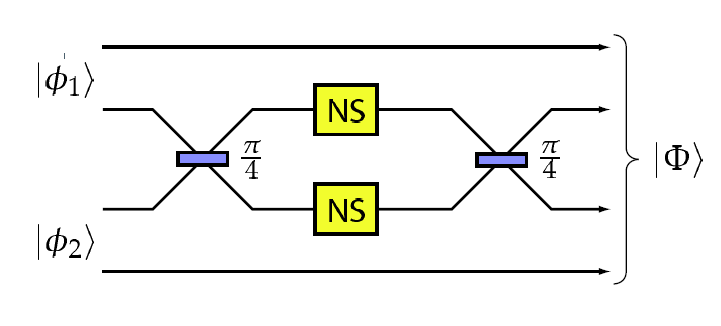
\includegraphics[width=0.9\textwidth]{images/CZ-gate.png}
    \caption{Circuit for probabilistic CZ gates in LOQC using NS gates}\label{fig:CZ_gate}
\end{figure}

As we can see in \ref{fig:CZ_gate}, when $\ket{\phi_1}$ and $\ket{\phi_2}$ are both equal to $\ket{1}$ then there will be a photon in the middle two modes ($\ket{\phi_2}$ is flipped). This means that the two photons will interact at the first beamsplitter, via the Hong-Ou-Mandel effect they will "bunch" and go down the same mode together towards the NS gate. The NS gate will sign shift the photons in the mode they went down due to the NS evolution \ref{NS evolution} and then the photons will interact with the second beamsplitter to finally give the state $-\ket{1,1}$.%\textbf{EVERYTHING AFTER THIS IS WRONG} What makes this circuit interesting is that because of the HOM effect, this situation only occurs when $\ket{\phi_1}$ and $\ket{\phi_2}$ are both equal to $\ket{1}$. In the case where only one photon goes through the middle modes, the photon will be split by the beamsplitter into both modes, each mode will interact with the NS gate, acquiring a phase shift each but these phase shifts destructively cancel when the modes are brought together at the second beamsplitter and the HOM effect occurs again. Due to the fact that the NS gate has a 1/4th probability of operating correctly and this gate requires two in tandem, the probability of the CZ gate operating as we expect is $p_{CZ} = p_{NS}^2 $

\subsubsection{Nonlinear sign shift gate}
As stated above, the nonlinear sign shift gate is a very useful tool as its non-deterministic effects allow us to achieve maximally entangled states when we otherwise couldn't but how is the NS gate made? The circuit is actually fairly simple; it involves 2 ancillary modes, one with a photon present and the other without, 3 beamsplitters set at differing angles with no phase shift and then 2 "perfect" photon detectors. We can see this in \ref{fig:NS_gate}. Going through each case for this NS gate is quite exhaustive which we won't cover here but the important thing to note is that 1/4 of the time the fock states $\alpha\ket{0}$ and $\beta\ket{1}$ are left untouched and when two photons come through from $\phi$, $\gamma\ket{2} \rightarrow -\gamma\ket{2}$ 

\begin{figure}[H]
    \centering
    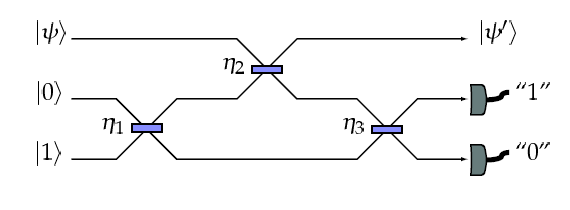
\includegraphics[width=0.9\textwidth]{images/NS gate.png}
    \caption{Circuit for probabilistic NS gates in LOQC using ancillary modes}\label{fig:NS_gate}
\end{figure}
%%%%%%%%%%%%%%%%%%%%%%%%%%%%%%%%%%%%%%%%%%



\subsection{Efficiency}
As we know by now, the real magic of quantum computation occurs when we can implement two-qubit gates as this allows us to perform quantum entanglement between qubit states which is then instrumental in many other constructs such as Quantum Teleportation, Quantum Algorithms, etc.

The issue we tend to run across with LOQC is that photons tend to not naturally interact with each other. This makes the practical implementation of a two-qubit gate a very difficult task. One suggested method is to use nonlinear Kerr media to provide a cross-phase modulation of $\pi$ between photon states. This combined with a beamsplitter can be used to construct a CNOT gate, from which a universal set of gates can be obtained. However, as stated in Section 7.4.3 in \cite{nielsen_chuang_2010}, obtaining nonlinear Kerr media with sufficient cross-phase modulation is not possible without incurring an excessive absorption loss: for every photon that incurs a $\pi$ cross-phase modulation, approximately 50 photons must be absorbed. Another suggested method of overcoming this uses photo-detectors to make projective measurements which can induce an interaction between photons\cite{Kok:2005jip}. This is a probabilistic approach with the probability of success being rather small and the more probabilistic photo-detectors (or non-deterministic operations in general) that are used, the probability of success for the entire circuit decreases exponentially. This makes optical computation seem quite unfeasible on the large scale but thanks to a few interesting results in quantum optics we can implement what is referred to as the KLM protocol to construct scalable 2-qubit gates.

\subsection{Scalability and the KLM Protocol}
As you probably might have guessed by now, there is a major problem with photonic quantum computing as we've discussed that uses probabilistic gates and that is the fact that the probabilities of these gates are quite low. Having a CZ gate that only works 1/nth of the time means that to get some reasonable result we need to run our circuit n times. As we implement more complicated circuits that involve some number, n, of deterministic gates with probabilities $\frac{1}{p}$, the chance of success of our circuit is $\frac{1}{p^n}$. This is obviously infeasible as any interesting circuit will require many gates and with our current set-up that means any scalable photonic quantum computer is too resource intensive to be worth it. \par
This alone sounds like it would be the nail in the coffin for further development into LOQC's but using quantum teleportation, the discrete quantum Fourier transform, and n number of photonic modes the probability of success for a given non-deterministic gate can become 'near-deterministic' with a success rate of $\frac{n^2}{(n+1)^2}$ which tends to 1 as n becomes sufficiently large. This is a process named the KLM protocol after Knill, Leflamme, and Milburn it was developed in 2000 and it is essential for any photonic quantum computer we could hope to build on a scale larger than a few gates.

\subsubsection{How does Quantum Teleportation work?}
Before we can get into how the KLM procedure works for near-deterministic photonic quantum computers we need to look at the phenomenon known as Quantum Teleportation. Unlike the name suggests, quantum teleportation does not involve 'teleporting' qubits in the common sense of the word; quantum teleportation is actually the process of transferring the exact state of one qubit to another. To expound upon this, quantum teleportation is the process of taking the initial state $\ket{\phi}_a = \alpha\ket{0} + \beta\ket{1}$ for some qubit \textit{a} and transferring it into some qubit \textit{b}. Quantum teleportation is limited in that information transfer (or in this case, 'teleportation') can not occur faster than light and due to the no-cloning theorem, the original qubit state is erased when being teleported to the second.
\par
We initially start with 2 entangled qubits being prepared by Eve. Eve then passes one of the entangled qubits to Alice and the other to Bob. Alice also has the initial qubit in state $\ket{\phi_j}$ that she wants to teleport to Bob. Alice then performs a Bell Basis Measurement across her two qubits and then classically sends information about the outcome of that measurement to Bob. Bob then performs one of 4 computations to his qubit from Eve and after this Bob will have the state $\ket{\phi_j}$. Before any of this can happen though, Alice has to perform a Bell Basis Measurement. \\
We first saw Bell states in  \ref{eqn:entqubit} but there are a total 4 Bell states (or EPR pairs) that represent 4 sets of 2 maximally entangled qubits. These states are:
\begin{align}\label{eqn:Bell States}
    B_0 &= \frac{1}{\sqrt{2}}\ket{00} + \ket{11} \\
    B_1 &= \frac{1}{\sqrt{2}}\ket{10} + \ket{01} \\
    B_2 &= \frac{1}{\sqrt{2}}\ket{00} - \ket{11} \\
    B_3 &= \frac{1}{\sqrt{2}}\ket{10} - \ket{01} \\
\end{align}
where from here on out we'll omit the factor of $\frac{1}{\sqrt{2}}$ and the order of labeling of $B_n$ doesn't actually matter but we've chosen this way for simplicity. 
\par
A Bell Basis Measurement is what happens when we take an arbitrary 2 qubit state and project it onto one of the four bases listed above. As mentioned in \ref{sec:USoQG} this can be as simple as applying a Hadamard and a CNOT. So Alice takes her initial qubit $\ket{\phi_j} = \alpha\ket{0} + \beta\ket{1}$ and performs a Bell Basis Measurement over it with the entangled qubit received from Eve. Mathematically this looks like:
\begin{align} \label{eqn:Bells QT}
    (\ket{00} + \ket{11})(\alpha\ket{0} + \beta\ket{1}) = \alpha\ket{000} + \beta\ket{001} + \alpha\ket{110} + \beta\ket{111}
\end{align}
where in the above equation, the state $\ket{101}$ would mean Alice's 2 qubits are in the state $\ket{01}$ (the first being in 1 and the second being in 0) and Bobs is in $\ket{1}$. Remember that when reading the states of qubits we look from right to left. 
\\
By performing the Bell Basis Measurement we project \ref{eqn:Bells QT} onto the states in \ref{eqn:Bell States}:
\begin{align}\label{eqn:final BM states}
    \alpha\ket{000} + \beta\ket{001} + \alpha\ket{110} + \beta\ket{111} = (\alpha\ket{0} + \beta\ket{1})B_0 + (\alpha\ket{1} + \beta\ket{0})B_1 \\ +(\alpha\ket{0} - \beta\ket{1})B_2 + (\alpha\ket{1} - \beta\ket{0})B_3 
\end{align}

We can see in \ref{eqn:final BM states}, when Alice looks at her qubits, if she sees $B_0$, the leftover state in Bob's qubit is $\alpha\ket{0} + \beta\ket{1} \equiv \ket{\phi_j}$. Teleportation has occurred and no further action is required. If Alice sees $B_1$ then the leftover state in Bob's qubit is $(\alpha\ket{1} + \beta\ket{0}) \equiv X\ket{\phi_j}$ where X represents the Pauli-X gate/ the quantum not gate operator $
\begin{pmatrix}
    0 & 1\\
    1 & 0\\
\end{pmatrix}$. If Alice sees $B_2$ then the leftover state in Bob's qubit is $(\alpha\ket{0} - \beta\ket{1}) \equiv Z\ket{\phi_j}$ where Z represents the Pauli Z gate (the Phase gate shown in \ref{eqn:phase} if $\phi = \pi$). Finally, if Alice sees $B_3$ then the leftover state in Bob's qubit is $(\alpha\ket{1} - \beta\ket{0}) \equiv ZX\ket{\phi_j}$. 
\\
Since the Z and X gates are their own inverses, all Bob has to do is wait for Alice to communicate classically, which of the 4 states she observed and then apply the $\mathbb{I}$, X, Z or XZ gates to his qubit to get the initial qubit $\ket{\phi_j}$. This is all shown diagrammatically in \ref{fig:QT circuit}

\begin{figure}[h]
    \centering
    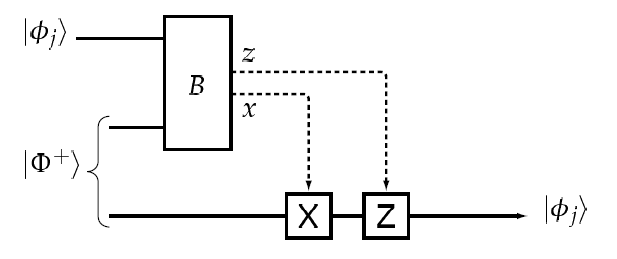
\includegraphics[width=0.9\textwidth]{images/QT circuit.png}
    \caption{Quantum teleportation circuit where the state $\phi_j$ is teleported to the second qubit. The bell measurement B gives one of 4 possibilities denoted $I, X, Z$, and $XZ$. The outcome is 'sent' classically (or in this case, we just measure what the outcome is) and then the corresponding gate is applied to the second qubit; the identity (nothing is done), the X gate (otherwise known as the not gate), the Z gate (otherwise known as the phase shifter), or the X followed by Z}\label{fig:QT circuit}
\end{figure}

\subsubsection{How Teleportation can be used in CZ gates}
Now that we understand how quantum teleportation works in theory, we now want to implement this with our non-deterministic CZ gate to see if we can improve our probability of success.
\par 
The first thing we must note is that the CZ gate operates on two qubits and because our teleporter only outputs a single mode, we need to double the circuit \ref{fig:QT circuit}, this looks like \ref{fig:QTCZ-1}. Now thanks to the fact that the CZ gate and the Pauli gates are in the Clifford group, we can commute the CZ gate with our X and Z gate operations (with some corrections) to achieve a circuit that is identical to \ref{fig:QTCZ-1} in output. This looks like \ref{fig:QTCZ-2} where the dashed X and Z boxes represent applying some combination of X and Z gates depending on the outcomes of the Bell Measurement. We can see a more comprehensive look at this in the Appendix\ref{Appendix}. The important takeaway from this is that we can apply a CZ gate to our inner modes in $\ket{\Phi^+}$, as shown in \ref{fig:QTCZ-2}, \textbf{before} the states $\ket{\phi_1}$ and $\ket{\phi_2}$ are teleported into these modes. This means that if we can prepare a successful $\ket{\Phi^+}$ 'offline', meaning before we put it into our circuit and perform teleportation we run $\ket{\Phi^+}$ multiple times until we have a successful result, then we can apply the teleportation when, and only when we have a successful $\ket{\Phi^+}$. This is significant because in \ref{fig:QTCZ-1} if the CZ gate fails then we have lost the states $\ket{\phi_1}$ and $\ket{\phi_2}$ so the probability of this circuit being correct hinges entirely on the CZ gate \textbf{but} in \ref{fig:QTCZ-2}, if everything highlighted in green is prepared offline, $\ket{\phi_1}$ and $\ket{\phi_2}$ are only teleported after a successful CZ gate operation, we essentially guarantee the success of the entire circuit in \ref{fig:QTCZ-2} and input states aren't destroyed.
\par
Unfortunately, there's a catch that we've neglected to mention up until now; performing a Bell Measurement is non-deterministic with a probability of $\frac{1}{2}$. Since we perform two Bell Measurements to teleport our two qubit states, the total probability of success for the \ref{fig:QTCZ-2} circuit is $\frac{1}{4}$ which is exactly what we started with. This is where the KLM near-deterministic teleporter comes in. 



%##############################
\begin{figure}
    \centering
\tikzset{every picture/.style={line width=0.75pt}} %set default line width to 0.75pt        

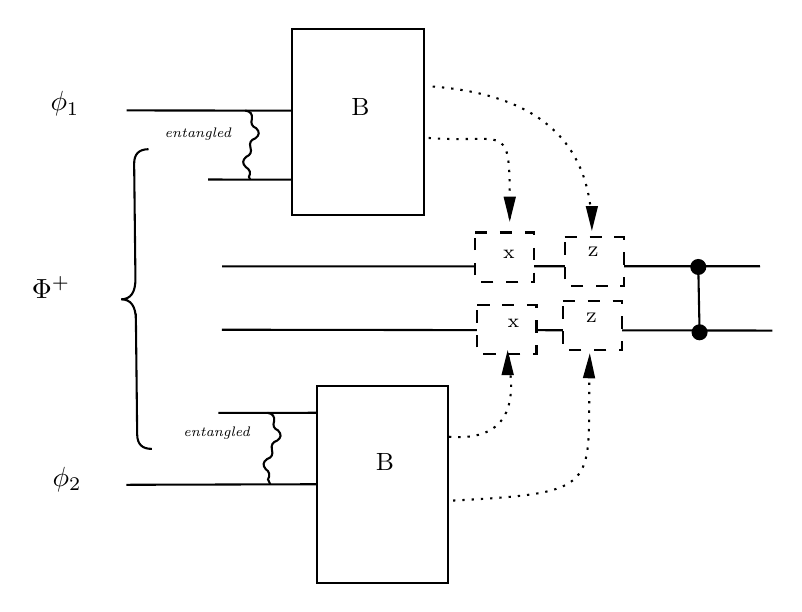
\begin{tikzpicture}[x=0.75pt,y=0.75pt,yscale=-1,xscale=1]
%uncomment if require: \path (0,300); %set diagram left start at 0, and has height of 300

%Shape: Brace [id:dp4160546662329181] 
\draw   (107.72,84.61) .. controls (103.05,84.66) and (100.75,87.02) .. (100.8,91.69) -- (101.42,146.88) .. controls (101.49,153.55) and (99.2,156.91) .. (94.53,156.96) .. controls (99.2,156.91) and (101.57,160.21) .. (101.64,166.88)(101.61,163.88) -- (102.26,222.08) .. controls (102.31,226.75) and (104.67,229.05) .. (109.34,229) ;
%Straight Lines [id:da8065384733259011] 
\draw    (97.23,65.94) -- (176.98,66.04) ;
%Shape: Rectangle [id:dp6790608484549128] 
\draw   (176.98,26.57) -- (240.39,26.57) -- (240.39,116.25) -- (176.98,116.25) -- cycle ;
%Straight Lines [id:da34073899408201536] 
\draw    (136.45,99.22) -- (176.98,99.32) ;
%Straight Lines [id:da3326977952142205] 
\draw    (97.07,246.31) -- (188.75,246.04) ;
%Shape: Rectangle [id:dp4807359036219334] 
\draw   (188.75,293.6) -- (252.15,293.6) -- (252.15,198.6) -- (188.75,198.6) -- cycle ;
%Straight Lines [id:da5430962616562778] 
\draw    (141.33,211.67) -- (188.75,211.61) ;
%Straight Lines [id:da9639318872173184] 
\draw    (143.18,141.07) -- (402.33,141) ;
%Straight Lines [id:da22467135117490433] 
\draw    (143.02,171.59) -- (408.33,172) ;
%Shape: Rectangle [id:dp5224143658365781] 
\draw  [fill={rgb, 255:red, 255; green, 255; blue, 255 }  ,fill opacity=1 ][dash pattern={on 4.5pt off 4.5pt}] (265.03,124.76) -- (293.66,124.76) -- (293.66,148.4) -- (265.03,148.4) -- cycle ;
%Shape: Rectangle [id:dp30201259432122174] 
\draw  [fill={rgb, 255:red, 255; green, 255; blue, 255 }  ,fill opacity=1 ][dash pattern={on 4.5pt off 4.5pt}] (307.38,157.82) -- (336.01,157.82) -- (336.01,181.45) -- (307.38,181.45) -- cycle ;
%Shape: Rectangle [id:dp20575966558705927] 
\draw  [fill={rgb, 255:red, 255; green, 255; blue, 255 }  ,fill opacity=1 ][dash pattern={on 4.5pt off 4.5pt}] (308.19,126.86) -- (336.82,126.86) -- (336.82,150.49) -- (308.19,150.49) -- cycle ;
%Shape: Rectangle [id:dp879155044923984] 
\draw  [fill={rgb, 255:red, 255; green, 255; blue, 255 }  ,fill opacity=1 ][dash pattern={on 4.5pt off 4.5pt}] (266.01,159.59) -- (294.64,159.59) -- (294.64,183.23) -- (266.01,183.23) -- cycle ;
%Curve Lines [id:da09246323435174553] 
\draw  [dash pattern={on 0.84pt off 2.51pt}]  (242.67,79.2) .. controls (282.34,82.32) and (281.78,68.69) .. (281.77,117.99) ;
\draw [shift={(281.76,119.5)}, rotate = 270] [fill={rgb, 255:red, 0; green, 0; blue, 0 }  ][line width=0.08]  [draw opacity=0] (12,-3) -- (0,0) -- (12,3) -- cycle    ;
%Curve Lines [id:da06959625459364571] 
\draw  [dash pattern={on 0.84pt off 2.51pt}]  (244.64,54.43) .. controls (284.31,57.55) and (320.6,72.61) .. (321.32,122.48) ;
\draw [shift={(321.33,124)}, rotate = 270] [fill={rgb, 255:red, 0; green, 0; blue, 0 }  ][line width=0.08]  [draw opacity=0] (12,-3) -- (0,0) -- (12,3) -- cycle    ;
%Curve Lines [id:da39316974650838654] 
\draw  [dash pattern={on 0.84pt off 2.51pt}]  (252.48,223.17) .. controls (289.95,226.11) and (282.09,193.82) .. (280.92,183.28) ;
\draw [shift={(280.78,181.42)}, rotate = 90] [fill={rgb, 255:red, 0; green, 0; blue, 0 }  ][line width=0.08]  [draw opacity=0] (12,-3) -- (0,0) -- (12,3) -- cycle    ;
%Curve Lines [id:da18722309143811278] 
\draw  [dash pattern={on 0.84pt off 2.51pt}]  (254.44,253.9) .. controls (329.57,250.04) and (318.6,247.3) .. (320.28,184.91) ;
\draw [shift={(320.33,183)}, rotate = 91.75] [fill={rgb, 255:red, 0; green, 0; blue, 0 }  ][line width=0.08]  [draw opacity=0] (12,-3) -- (0,0) -- (12,3) -- cycle    ;
%Straight Lines [id:da761825964657918] 
\draw    (372.6,141.36) -- (373.22,172.83) ;
\draw [shift={(373.22,172.83)}, rotate = 88.87] [color={rgb, 255:red, 0; green, 0; blue, 0 }  ][fill={rgb, 255:red, 0; green, 0; blue, 0 }  ][line width=0.75]      (0, 0) circle [x radius= 3.35, y radius= 3.35]   ;
\draw [shift={(372.6,141.36)}, rotate = 88.87] [color={rgb, 255:red, 0; green, 0; blue, 0 }  ][fill={rgb, 255:red, 0; green, 0; blue, 0 }  ][line width=0.75]      (0, 0) circle [x radius= 3.35, y radius= 3.35]   ;
%Curve Lines [id:da1435143281948974] 
\draw    (165.04,211.64) .. controls (167.55,212.01) and (168.61,213.36) .. (168.22,215.68) .. controls (167.48,217.79) and (168.12,219.27) .. (170.14,220.12) .. controls (171.89,221.97) and (171.73,223.6) .. (169.67,225.03) .. controls (167.48,225.7) and (166.66,227.19) .. (167.2,229.5) .. controls (167.82,231.73) and (167.06,233.19) .. (164.92,233.87) .. controls (162.85,235.26) and (162.59,236.87) .. (164.16,238.71) .. controls (166.02,239.98) and (166.4,241.65) .. (165.3,243.72) -- (166.33,246) ;
%Curve Lines [id:da2586024030465792] 
\draw    (154.33,66) .. controls (156.84,66.37) and (157.91,67.71) .. (157.54,70.02) .. controls (156.85,72.15) and (157.53,73.65) .. (159.6,74.52) .. controls (161.38,76.25) and (161.23,77.88) .. (159.16,79.43) .. controls (156.98,80.08) and (156.2,81.51) .. (156.82,83.74) .. controls (157.55,85.92) and (156.87,87.44) .. (154.8,88.29) .. controls (152.9,89.89) and (152.84,91.54) .. (154.61,93.24) .. controls (156.62,94.44) and (157.12,96.02) .. (156.1,97.98) -- (156.72,99.27) ;

% Text Node
\draw (279.19,165.08) node [anchor=north west][inner sep=0.75pt]  [font=\normalsize] [align=left] {{\scriptsize x}};
% Text Node
\draw (277.03,131.76) node [anchor=north west][inner sep=0.75pt]  [font=\normalsize] [align=left] {{\scriptsize x}};
% Text Node
\draw (316.87,162.09) node [anchor=north west][inner sep=0.75pt]   [align=left] {{\tiny Z}};
% Text Node
\draw (317.71,130.36) node [anchor=north west][inner sep=0.75pt]   [align=left] {{\tiny Z}};
% Text Node
\draw (204.01,58.73) node [anchor=north west][inner sep=0.75pt]  [font=\normalsize] [align=left] {{\small B}};
% Text Node
\draw (215.78,229.78) node [anchor=north west][inner sep=0.75pt]  [font=\normalsize] [align=left] {{\small B}};
% Text Node
\draw (59,55.4) node [anchor=north west][inner sep=0.75pt]    {$\ket{\phi _{1}}$};
% Text Node
\draw (60,236.4) node [anchor=north west][inner sep=0.75pt]    {$\ket{\phi _{2}}$};
% Text Node
\draw (123,217) node [anchor=north west][inner sep=0.75pt]   [align=left] {\textit{{\tiny entangled}}};
% Text Node
\draw (114,73) node [anchor=north west][inner sep=0.75pt]   [align=left] {\textit{{\tiny entangled}}};
% Text Node
\draw (50,144.4) node [anchor=north west][inner sep=0.75pt]    {$\ket{\Phi ^{+}}$};


\end{tikzpicture}
    \caption{A circuit where quantum teleportation is used just before a CZ-gate is applied. The states $\ket{\phi_1}$ and $\ket{\phi_2}$ are teleported into the middle 2 modes using the Bell Measurement B, and the operations X and Z are applied to the middle two modes depending on the Bell Measurement made. If the CZ gate has a probability of success of $\frac{1}{4}$ then the probability of losing the states $\ket{\phi_1}$ and $\ket{\phi_2}$ is $\frac{3}{4}$. It should be noted that this figure is equivalent to \ref{fig:QTCZ-2}. To see this proof see \ref{Appendix}}
    \label{fig:QTCZ-1}
\end{figure}

%#############################
\begin{figure}[!h]
\centering


\tikzset{every picture/.style={line width=0.75pt}} %set default line width to 0.75pt        

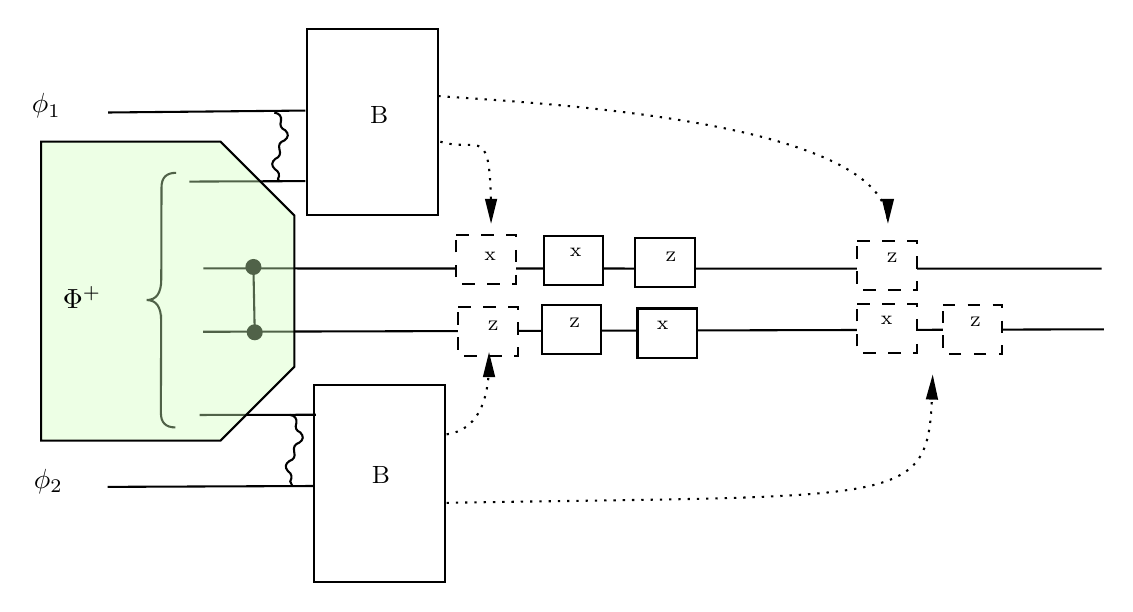
\begin{tikzpicture}[x=0.75pt,y=0.75pt,yscale=-1,xscale=1]
%uncomment if require: \path (0,300); %set diagram left start at 0, and has height of 300

%Shape: Brace [id:dp4160546662329181] 
\draw   (130,95) .. controls (125.33,94.99) and (122.99,97.31) .. (122.98,101.98) -- (122.86,146.31) .. controls (122.84,152.98) and (120.5,156.3) .. (115.83,156.29) .. controls (120.5,156.3) and (122.82,159.64) .. (122.8,166.31)(122.81,163.31) -- (122.68,210.65) .. controls (122.67,215.32) and (124.99,217.66) .. (129.66,217.67) ;
%Straight Lines [id:da8065384733259011] 
\draw    (97.23,65.94) -- (192.33,65) ;
%Shape: Rectangle [id:dp6790608484549128] 
\draw   (192.98,25.57) -- (256.39,25.57) -- (256.39,115.25) -- (192.98,115.25) -- cycle ;
%Straight Lines [id:da34073899408201536] 
\draw    (136.45,99.22) -- (192.33,99) ;
%Straight Lines [id:da3326977952142205] 
\draw    (97.07,246.31) -- (196.33,245.89) ;
%Shape: Rectangle [id:dp4807359036219334] 
\draw   (196.33,292.34) -- (259.74,292.34) -- (259.74,197.33) -- (196.33,197.33) -- cycle ;
%Straight Lines [id:da5430962616562778] 
\draw    (141.33,211.67) -- (197.33,211.56) ;
%Straight Lines [id:da9639318872173184] 
\draw    (143.18,141.07) -- (575.92,141.17) ;
%Straight Lines [id:da22467135117490433] 
\draw    (143.02,171.59) -- (577,170.4) ;
%Shape: Rectangle [id:dp4475966088803329] 
\draw  [fill={rgb, 255:red, 255; green, 255; blue, 255 }  ,fill opacity=1 ] (307.19,125.54) -- (335.82,125.54) -- (335.82,149.17) -- (307.19,149.17) -- cycle ;
%Shape: Rectangle [id:dp01609794668273845] 
\draw  [fill={rgb, 255:red, 255; green, 255; blue, 255 }  ,fill opacity=1 ] (306.21,158.82) -- (334.84,158.82) -- (334.84,182.45) -- (306.21,182.45) -- cycle ;
%Shape: Rectangle [id:dp456238595830335] 
\draw  [fill={rgb, 255:red, 255; green, 255; blue, 255 }  ,fill opacity=1 ] (351.32,126.31) -- (379.95,126.31) -- (379.95,149.94) -- (351.32,149.94) -- cycle ;
%Shape: Rectangle [id:dp6950101334971088] 
\draw  [fill={rgb, 255:red, 255; green, 255; blue, 255 }  ,fill opacity=1 ] (352.3,160.37) -- (380.93,160.37) -- (380.93,184) -- (352.3,184) -- cycle ;
%Shape: Rectangle [id:dp5224143658365781] 
\draw  [fill={rgb, 255:red, 255; green, 255; blue, 255 }  ,fill opacity=1 ][dash pattern={on 4.5pt off 4.5pt}] (265.03,124.76) -- (293.66,124.76) -- (293.66,148.4) -- (265.03,148.4) -- cycle ;
%Shape: Rectangle [id:dp8276974594794448] 
\draw  [fill={rgb, 255:red, 255; green, 255; blue, 255 }  ,fill opacity=1 ][dash pattern={on 4.5pt off 4.5pt}] (458.19,158.05) -- (486.82,158.05) -- (486.82,181.68) -- (458.19,181.68) -- cycle ;
%Shape: Rectangle [id:dp30201259432122174] 
\draw  [fill={rgb, 255:red, 255; green, 255; blue, 255 }  ,fill opacity=1 ][dash pattern={on 4.5pt off 4.5pt}] (499.38,158.82) -- (528.01,158.82) -- (528.01,182.45) -- (499.38,182.45) -- cycle ;
%Shape: Rectangle [id:dp20575966558705927] 
\draw  [fill={rgb, 255:red, 255; green, 255; blue, 255 }  ,fill opacity=1 ][dash pattern={on 4.5pt off 4.5pt}] (458.19,127.86) -- (486.82,127.86) -- (486.82,151.49) -- (458.19,151.49) -- cycle ;
%Shape: Rectangle [id:dp879155044923984] 
\draw  [fill={rgb, 255:red, 255; green, 255; blue, 255 }  ,fill opacity=1 ][dash pattern={on 4.5pt off 4.5pt}] (266.01,159.59) -- (294.64,159.59) -- (294.64,183.23) -- (266.01,183.23) -- cycle ;
%Curve Lines [id:da09246323435174553] 
\draw  [dash pattern={on 0.84pt off 2.51pt}]  (257.33,80) .. controls (277.13,85.94) and (281.67,68.76) .. (281.76,117.99) ;
\draw [shift={(281.76,119.5)}, rotate = 270] [fill={rgb, 255:red, 0; green, 0; blue, 0 }  ][line width=0.08]  [draw opacity=0] (12,-3) -- (0,0) -- (12,3) -- cycle    ;
%Curve Lines [id:da06959625459364571] 
\draw  [dash pattern={on 0.84pt off 2.51pt}]  (256.33,58) .. controls (296,61.12) and (469.45,68.27) .. (472.91,117.98) ;
\draw [shift={(472.97,119.5)}, rotate = 270] [fill={rgb, 255:red, 0; green, 0; blue, 0 }  ][line width=0.08]  [draw opacity=0] (12,-3) -- (0,0) -- (12,3) -- cycle    ;
%Curve Lines [id:da39316974650838654] 
\draw  [dash pattern={on 0.84pt off 2.51pt}]  (260.33,221) .. controls (280.79,218.21) and (280.89,193.07) .. (280.8,183.34) ;
\draw [shift={(280.78,181.42)}, rotate = 90] [fill={rgb, 255:red, 0; green, 0; blue, 0 }  ][line width=0.08]  [draw opacity=0] (12,-3) -- (0,0) -- (12,3) -- cycle    ;
%Curve Lines [id:da18722309143811278] 
\draw  [dash pattern={on 0.84pt off 2.51pt}]  (260.33,254) .. controls (492.98,250.04) and (492.61,256.37) .. (494.48,194.16) ;
\draw [shift={(494.54,192.26)}, rotate = 91.75] [fill={rgb, 255:red, 0; green, 0; blue, 0 }  ][line width=0.08]  [draw opacity=0] (12,-3) -- (0,0) -- (12,3) -- cycle    ;
%Straight Lines [id:da761825964657918] 
\draw    (167.26,140.36) -- (167.89,171.83) ;
\draw [shift={(167.89,171.83)}, rotate = 88.87] [color={rgb, 255:red, 0; green, 0; blue, 0 }  ][fill={rgb, 255:red, 0; green, 0; blue, 0 }  ][line width=0.75]      (0, 0) circle [x radius= 3.35, y radius= 3.35]   ;
\draw [shift={(167.26,140.36)}, rotate = 88.87] [color={rgb, 255:red, 0; green, 0; blue, 0 }  ][fill={rgb, 255:red, 0; green, 0; blue, 0 }  ][line width=0.75]      (0, 0) circle [x radius= 3.35, y radius= 3.35]   ;
%Curve Lines [id:da1435143281948974] 
\draw    (184.75,211.61) .. controls (187.26,211.98) and (188.32,213.33) .. (187.93,215.65) .. controls (187.19,217.76) and (187.83,219.24) .. (189.85,220.09) .. controls (191.59,221.94) and (191.43,223.57) .. (189.37,225) .. controls (187.19,225.67) and (186.37,227.16) .. (186.91,229.47) .. controls (187.52,231.7) and (186.76,233.16) .. (184.63,233.84) .. controls (182.56,235.23) and (182.3,236.84) .. (183.87,238.68) .. controls (185.73,239.95) and (186.11,241.62) .. (185.01,243.69) -- (186.04,245.97) ;
%Curve Lines [id:da2586024030465792] 
\draw    (177.33,66) .. controls (179.84,66.37) and (180.91,67.71) .. (180.54,70.02) .. controls (179.85,72.15) and (180.53,73.65) .. (182.6,74.52) .. controls (184.38,76.25) and (184.23,77.88) .. (182.16,79.43) .. controls (179.98,80.08) and (179.2,81.51) .. (179.82,83.74) .. controls (180.55,85.92) and (179.87,87.44) .. (177.8,88.29) .. controls (175.9,89.89) and (175.84,91.54) .. (177.61,93.24) .. controls (179.62,94.44) and (180.12,96.02) .. (179.1,97.98) -- (179.72,99.27) ;
%Snip Same Side Corner Rect [id:dp59755192438972] 
\draw  [fill={rgb, 255:red, 208; green, 254; blue, 187 }  ,fill opacity=0.39 ] (151.42,80) -- (187,115.58) -- (187,188.42) -- (151.42,224) -- (65,224) -- (65,224) -- (65,80) -- (65,80) -- cycle ;

% Text Node
\draw (317.69,163.54) node [anchor=north west][inner sep=0.75pt]   [align=left] {{\tiny Z}};
% Text Node
\draw (364.12,131.88) node [anchor=north west][inner sep=0.75pt]   [align=left] {{\tiny Z}};
% Text Node
\draw (360.19,165.08) node [anchor=north west][inner sep=0.75pt]  [font=\normalsize] [align=left] {{\scriptsize x}};
% Text Node
\draw (318.2,129.83) node [anchor=north west][inner sep=0.75pt]  [font=\normalsize] [align=left] {{\scriptsize x}};
% Text Node
\draw (277.03,131.76) node [anchor=north west][inner sep=0.75pt]  [font=\normalsize] [align=left] {{\scriptsize x}};
% Text Node
\draw (510.87,163.09) node [anchor=north west][inner sep=0.75pt]   [align=left] {{\tiny Z}};
% Text Node
\draw (470.71,132.36) node [anchor=north west][inner sep=0.75pt]   [align=left] {{\tiny Z}};
% Text Node
\draw (468.12,162.73) node [anchor=north west][inner sep=0.75pt]  [font=\normalsize] [align=left] {{\scriptsize x}};
% Text Node
\draw (278.53,165.09) node [anchor=north west][inner sep=0.75pt]   [align=left] {{\tiny Z}};
% Text Node
\draw (222.01,61.73) node [anchor=north west][inner sep=0.75pt]  [font=\normalsize] [align=left] {{\small B}};
% Text Node
\draw (222.78,234.78) node [anchor=north west][inner sep=0.75pt]  [font=\normalsize] [align=left] {{\small B}};
% Text Node
\draw (59,55.4) node [anchor=north west][inner sep=0.75pt]    {$\ket{\phi _{1}}$};
% Text Node
\draw (60,236.4) node [anchor=north west][inner sep=0.75pt]    {$\ket{\phi _{2}}$};
% Text Node
\draw (74,148.4) node [anchor=north west][inner sep=0.75pt]    {$\ket{\Phi ^{+}}$};


\end{tikzpicture}


 \caption{A CZ-gate circuit that uses quantum teleportation. Using the fact that the CZ gate and the Pauli gates are in the Clifford group, we can commute the CZ gate with the X and Z gates (with some correction) such that this circuit is equivalent to \ref{fig:QTCZ-1}. See \ref{Appendix} for proof. Figure developed from SOURCE. }
    \label{fig:QTCZ-2}
\end{figure}

\subsubsection{KLM Near Deterministic Teleporter}
Due to the non-deterministic nature of the Bell Basis Measurement, the circuit \ref{fig:QTCZ-2} has a probability of success of $\frac{1}{4}$ but if there is a way we can deterministically (or near deterministically) teleport our input states $\ket{\phi_1}$ and $\ket{\phi_2}$ after a successful CZ gate (prepared offline) is implemented then we have a near deterministic CZ circuit.
\par
For this section alone we'll be considering the single-rail qubit representation as opposed to the dual-rail representation that we've been focused on until now because the CZ gate in single-rail encoding only requires one optical mode and so the picture here should be clearer to see when we teleport one optical mode. The aim is to teleport the initial qubit $\ket{\phi} = \alpha\ket{0} + \beta\ket{1}$.
\par
We start by preparing 2n optical modes and we're going to put them in the superposition state:
    \begin{equation}
        \ket{t_n} = \frac{1}{\sqrt{n+1}}\sum\limits_{j=0}^{n}\ket{1}^j\ket{0}^{n-j}\ket{0}^j\ket{1}^{n-j}
        \label{eqn: QFT Teleporter EQ}
    \end{equation}
here $\ket{k}^j \equiv \ket{k}_1 \otimes...\otimes\ket{k}_j$ where $\ket{k}_j$ signifies the $j^{th}$ mode being in the state $\ket{k}$ and $\otimes$ represents the tensor product. 
\par
We're going to look at an example where we choose n=5 to see what $\ket{t_n}$ looks like. Remembering that $\ket{t_n}$ represents 2n optical modes, $\ket{t_5}$ describes 10 optical modes.
\begin{equation}
        \ket{t_5} = \frac{1}{\sqrt{5+1}}\sum\limits_{j=0}^5\ket{1}^j\ket{0}^{5-j}\ket{0}^j\ket{1}^{5-j}
    \end{equation}
    \begin{align} 
        \ket{t_5} =  & \ket{0}^{5}\ket{1}^5 
        + \\ & \ket{1}\ket{0}^{4}\ket{0}\ket{1}^{4} + 
 \\ & \ket{1}^2\ket{0}^{3}\ket{0}^2\ket{1}^{3} \label{t5:1} + \\ & \ket{1}^3\ket{0}^{2}\ket{0}^3\ket{1}^{2}\label{t5:2} + \\  & \ket{1}^4\ket{0}\ket{0}^4\ket{1} + \\ & \ket{1}^{5}\ket{0}^5  
 \label{eqn: t5 breakdown}
\end{align}
\textit{note: we've neglected the preceding normalisation term for conciseness but each of the states in the $\ket{t_n}$ superposition have equal probability }
\par
If we look at just one of the lines above, \ref{eqn: t5 breakdown}, for example, $\ket{1}^5\ket{0}^5$ and explicitly write it as a string of 0's and 1's representing whether a photon is present in a given optical mode then if $\ket{t_5} = \ket{1}^5\ket{0}^5$:
    \begin{equation}
        \ket{t_5} = 1111100000
    \end{equation}
In this example the first 5 optical modes \footnote{and therefore the first 5 qubits since this is single-rail encoding} in $\ket{t_5}$ have a photon present whilst the latter 5 have none.
\par 
As you can see, $\ket{t_5}$ is a superposition of all of these states when we prepare it. In our near deterministic teleporter, we put the first n modes (in our example, the first 5) as well as the input mode $\ket{\phi}$ (the state we want to teleport) into the discrete Quantum Fourier Transform (QFT).  We haven't discussed the discrete QFT in detail and it goes beyond the scope of this report but there are two important results to know from applying it:
\begin{itemize}
    \item after inputting n+1 modes the QFT will output 1 singular mode with "m" photons
    \item these m photons come from our input modes but the information about which exact modes they came from is destroyed, the 'which-path' information is erased.
\end{itemize}
So after the input mode $\ket{phi}$ and the first n modes of $\ket{t_n}$ are put through the QFT, the output 'm' tells us there are m photons in these first n+1 modes, we then find that the $(n+m)^{th}$ mode has the exact state of $\ket{\phi}$. This is shown diagrammatically in \ref{fig:Near deterministic tele}. To see this clearly we go back to our example of $\ket{t_5}$.
\par
Imagine, after applying the QFT over $\ket{\phi} (= \alpha\ket{0} + \beta\ket{1}$) and $\ket{t_5}$, the output is m=3. Logically we know then that either 1 photon came from $\ket{\phi}$ (in which case the other 2 came from the first 5 modes of $\ket{t_5}$) or 0 photons came from $\ket{\phi}$ (in which case all 3 came from the first 5 modes of $\ket{t_5}$). Due to the QFT destroying 'which-path' information, we don't know which of these two cases our output corresponds to but we know it can only be one of these two. This means that the only contributions to $\ket{t_5}$ from our large sum are \ref{t5:1} and \ref{t5:2}. With the modes for each circuit written explicitly, these two possibilities are:
 \begin{alignat*}{0}
        &\mathbf{0} \quad  &  &\mathbf{1 2 3 4 5}  \quad &  &\mathbf{6 7 8 9 (10)}\\
        \alpha \;\;\;  &0 \quad &  &0 1 1 1 0 0  \quad  &  &1 1 {\color{red}0} 0 0 \\
        \beta  \;\;\; &1 \quad  &  &1 1 1 0 0 0 \quad &  &1 1 {\color{red}1} 0 0 \\
\end{alignat*}
where the bold numbers are labels for each mode and $\alpha$ and $\beta$ are the amplitudes for each possibility. The zeroth column represents our input qubit $\ket{\phi}$, columns 1-5 represent the first 5 modes of $\ket{t_5}$ and columns 6-10 represent the last 5 modes of $\ket{t_5}$.
\par
The 'teleportation' happens when we look at the $(n+m)^{th}$ mode, in our case this is the 8th column as highlighted in red above.  We can see that this column is exactly the same as the zeroth column (our input mode). We have just teleported our input mode into the 8th mode of our circuit. 
\par
As you might have guessed, our QFT is not deterministic, it fails when the output m is equal to 0 or n+1 because in these cases we know the input state $\ket{\phi}$ collapsed and there is only one possible outcome of the $\ket{t_5}$ superposition our circuit could be in but since these are only 2 cases if we increase the number of modes n, the chances of m= 0,(n+1) diminishes. More explicitly we can say that as we increase the number of modes in the circuit in \ref{fig:Near deterministic tele} the probability, $= \frac{n}{n+1}$, approaches one.

\begin{figure}
    \centering
    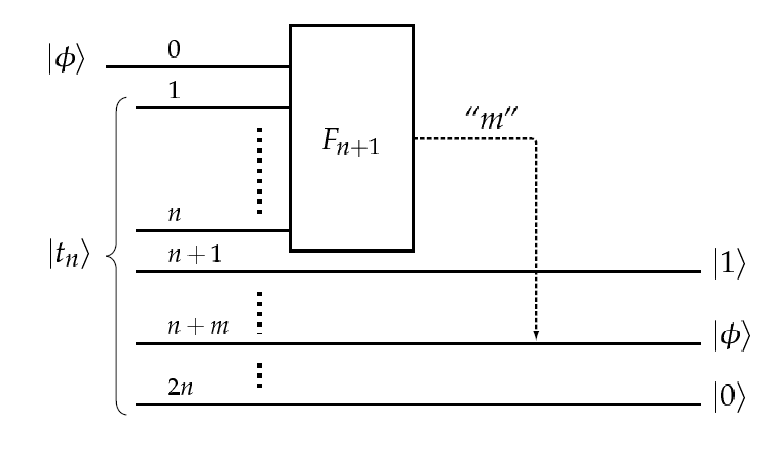
\includegraphics[scale=0.5]{images/Near Deterministic Teleporter.png}
    \caption{Near Deterministic Teleporter}
    \label{fig:Near deterministic tele}
\end{figure}

\subsection{Bringing it all together}
